\section{Funcionamiento}

\subsection{Servidor}
\begin{frame}{Servidor}
	\begin{block}{  }
		La interfaz del servidor es sencilla.
	\end{block}
	
	\begin{exampleblock}{ }
		\begin{figure}[H]
			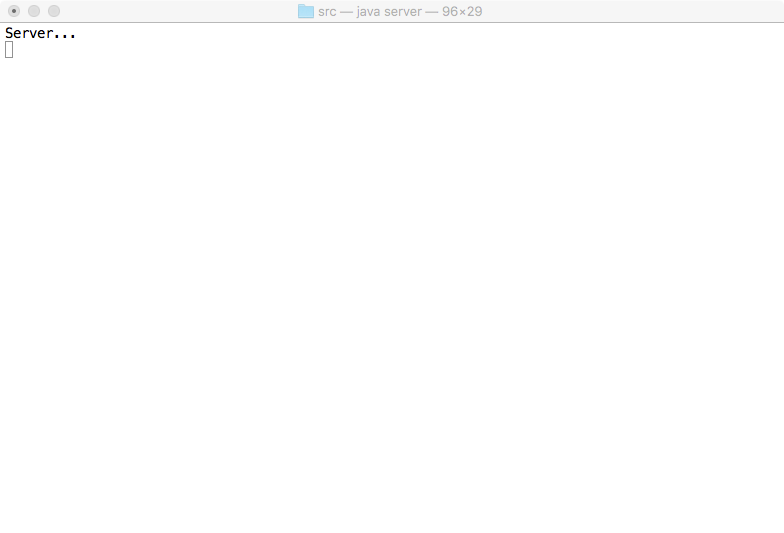
\includegraphics[scale=0.31]{./Imagenes/server1.png}
		\end{figure}
	\end{exampleblock}
\end{frame}


% -----------------------------------


\subsection{Cliente}
\begin{frame}{Usuario}
	\begin{block}{  }
		Cada usuario tiene un terminal para el Writer y otro para el Printer.
	\end{block}
	
	\begin{exampleblock}{Fran writer}
		\begin{figure}[H]
			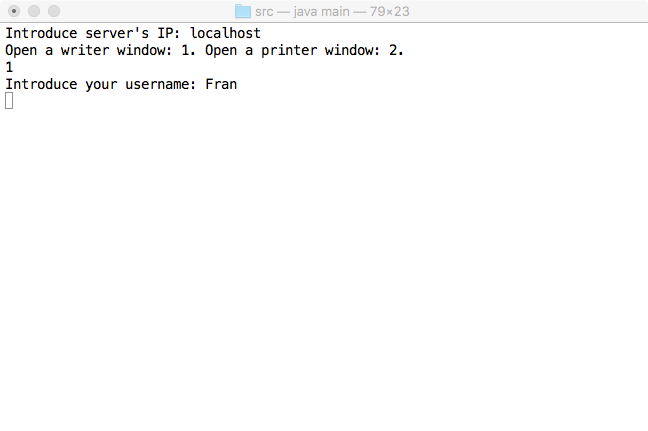
\includegraphics[scale=0.4]{./Imagenes/franwriter1.png}
		\end{figure}
	\end{exampleblock}
\end{frame}


% -----------------------------------


\begin{frame}{Usuario}
	\begin{block}{  }
		Cada usuario tiene un terminal para el Writer y otro para el Printer.
	\end{block}
	
	\begin{exampleblock}{Fran printer}
		\begin{figure}[H]
			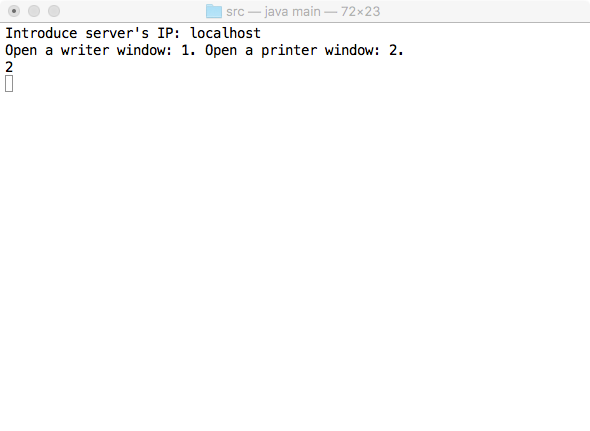
\includegraphics[scale=0.4]{./Imagenes/franprinter1.png}
		\end{figure}
	\end{exampleblock}
\end{frame}


% -----------------------------------


\begin{frame}{Usuario}
	\begin{block}{  }
		Cada usuario tiene un terminal para el Writer y otro para el Printer.
	\end{block}
	
	\begin{exampleblock}{Ruben writer}
		\begin{figure}[H]
			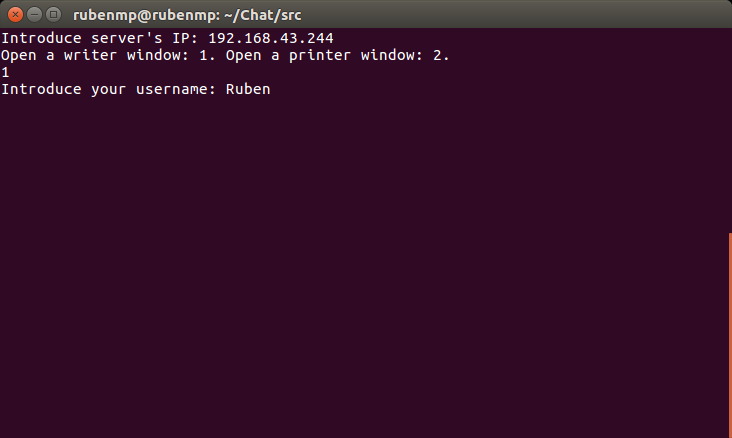
\includegraphics[scale=0.4]{./Imagenes/rubenwriter1.png}
		\end{figure}
	\end{exampleblock}
\end{frame}


% -----------------------------------


\begin{frame}{Usuario}
	\begin{block}{  }
		Cada usuario tiene un terminal para el Writer y otro para el Printer.
	\end{block}
	
	\begin{exampleblock}{Ruben printer}
		\begin{figure}[H]
			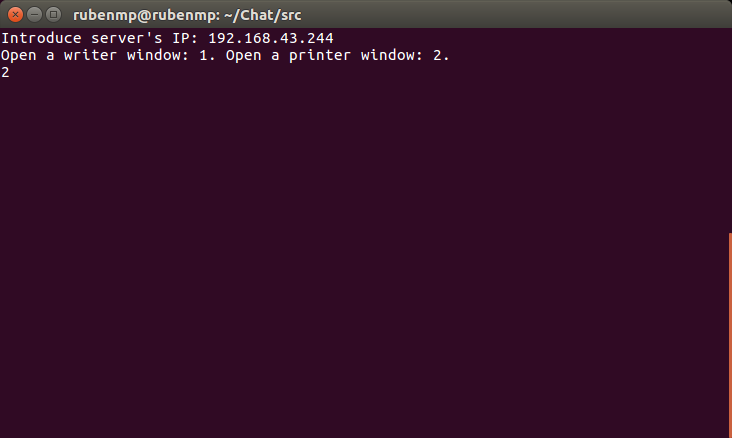
\includegraphics[scale=0.4]{./Imagenes/rubenprinter1.png}
		\end{figure}
	\end{exampleblock}
\end{frame}


% -----------------------------------


\subsection{Escribir mensajes}
\begin{frame}{Escribir mensajes}
	\begin{block}{ }
		Ahora procedemos a escribir mensajes desde ambos ordenadores.
	\end{block}
	
	\begin{exampleblock}{Ruben escribiendo}
		\begin{figure}[H]
			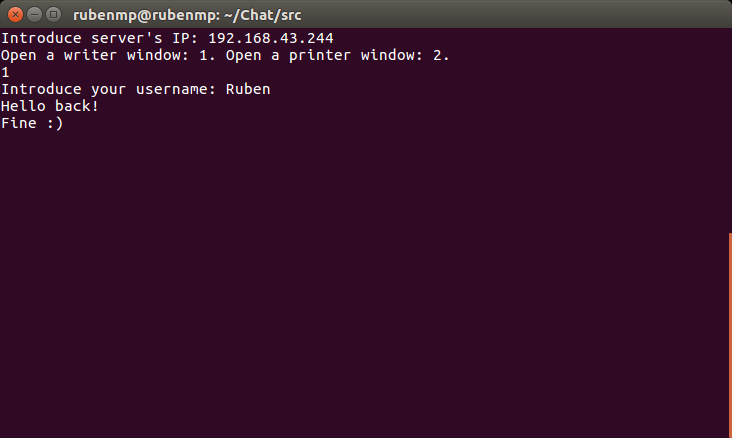
\includegraphics[scale=0.4]{./Imagenes/rubenwriter2.png}
		\end{figure}
	\end{exampleblock}
\end{frame}


% -----------------------------------


\begin{frame}{Escribir mensajes}
	\begin{block}{ }
		Ahora procedemos a escribir mensajes desde ambos ordenadores.
	\end{block}
	
	\begin{exampleblock}{Fran escribiendo}
		\begin{figure}[H]
			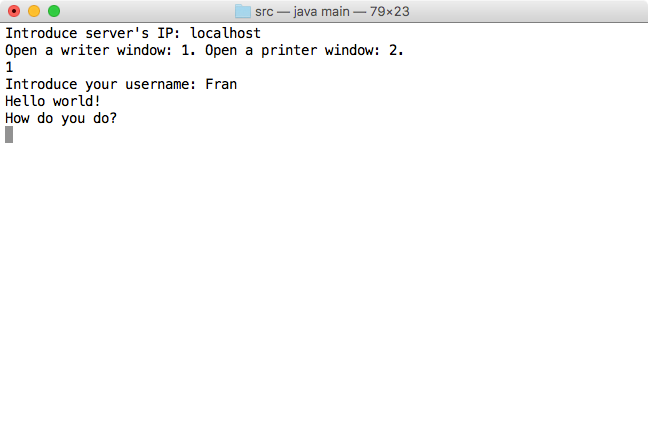
\includegraphics[scale=0.4]{./Imagenes/franwriter2.png}
		\end{figure}
	\end{exampleblock}
\end{frame}


% -----------------------------------


\begin{frame}{Escribir mensajes}
	\begin{block}{ }
		Comprobamos que funciona
	\end{block}
	
	\begin{exampleblock}{Fran recibiendo}
		\begin{figure}[H]
			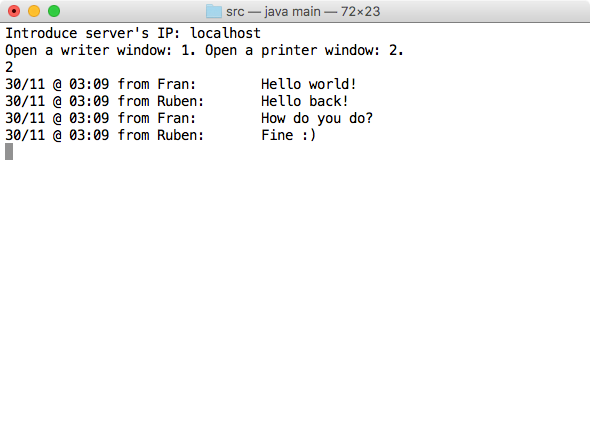
\includegraphics[scale=0.4]{./Imagenes/franprinter2.png}
		\end{figure}
	\end{exampleblock}
\end{frame}


% -----------------------------------


\begin{frame}{Escribir mensajes}
	\begin{block}{ }
		Comprobamos que funciona
	\end{block}
	
	\begin{exampleblock}{Ruben recibiendo}
		\begin{figure}[H]
			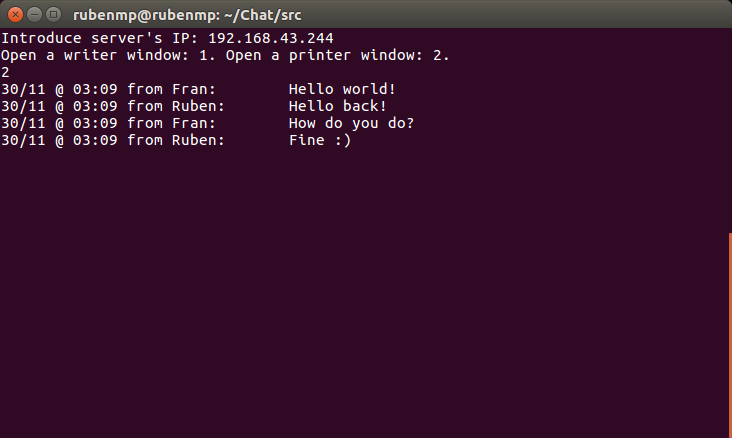
\includegraphics[scale=0.4]{./Imagenes/rubenprinter2.png}
		\end{figure}
	\end{exampleblock}
\end{frame}

